\chapter{Présentation générale}

\section*{Qu'est-ce que Slyum}

\texttt{Slyum} est un éditeur de diagramme de classes UML (Unified Modeling Language) conçu pour être simple à prendre en main et à utiliser. La figure ~\ref{img:main_screen} représente l'affichage classique de Slyum.

\begin{figure}[h]
	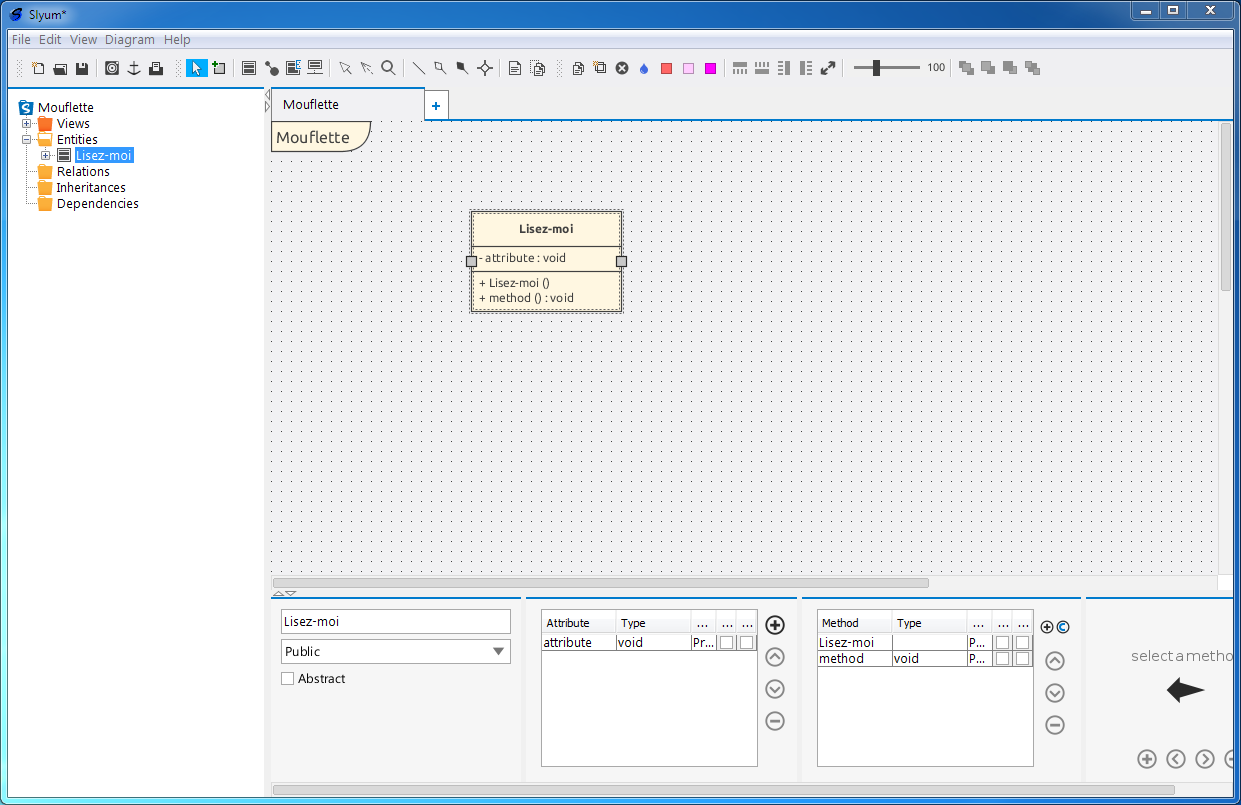
\includegraphics[width=\textwidth]{images/slyum-window.png}
	\caption{Capture d'écran de Slyum}
	\label{img:main_screen}
\end{figure}

\section*{Remarques, questions et bugs (à revoir)}

Pour tout report de problème, proposition d'amélioration ou de remarque, merci de vous rendre à l'adresse suivante:
https://github.com/HEIG-GAPS/slyum/issues.
Depuis cette interface, vous pouvez également voir les problème déjà reportés. Merci de vous assurez que le problème n'existe pas déjà avant d'en reporter un.